\styledchapter[Inleiding]{inleiding}

NGTI is een software ontwikkelbedrijf dat gevestigd is in Rotterdam. Opgericht in 2012 maakt NTGI applicaties (apps) voor mobiel en/of webgebruik. Naast het ontwikkelen werkt NGTI aan het hele traject om een app heen, namelijk de probleemstelling, mockups, wireframes en prototyping. Daarnaast levert NGTI ook support en lost bugs op nadat een app live is gegaan \cite{ngti-services}. Ook maakt NGTI white label apps en frameworks \cite{ngti-solutions}.

Het bedrijf heeft, zoals de meeste bedrijven, een organogram (\autoref{fig:ngti-organogram}). In de praktijk is dit echter niet terug te vinden en wordt de structuur gezien als "plat". Collega's kunnen elkaar laagdrempelig benaderen waardoor niemand een onbekende is en verschillende disciplines makkelijk met elkaar samen kunnen werken.  

\begin{figure}[hbt!]
  \centering
  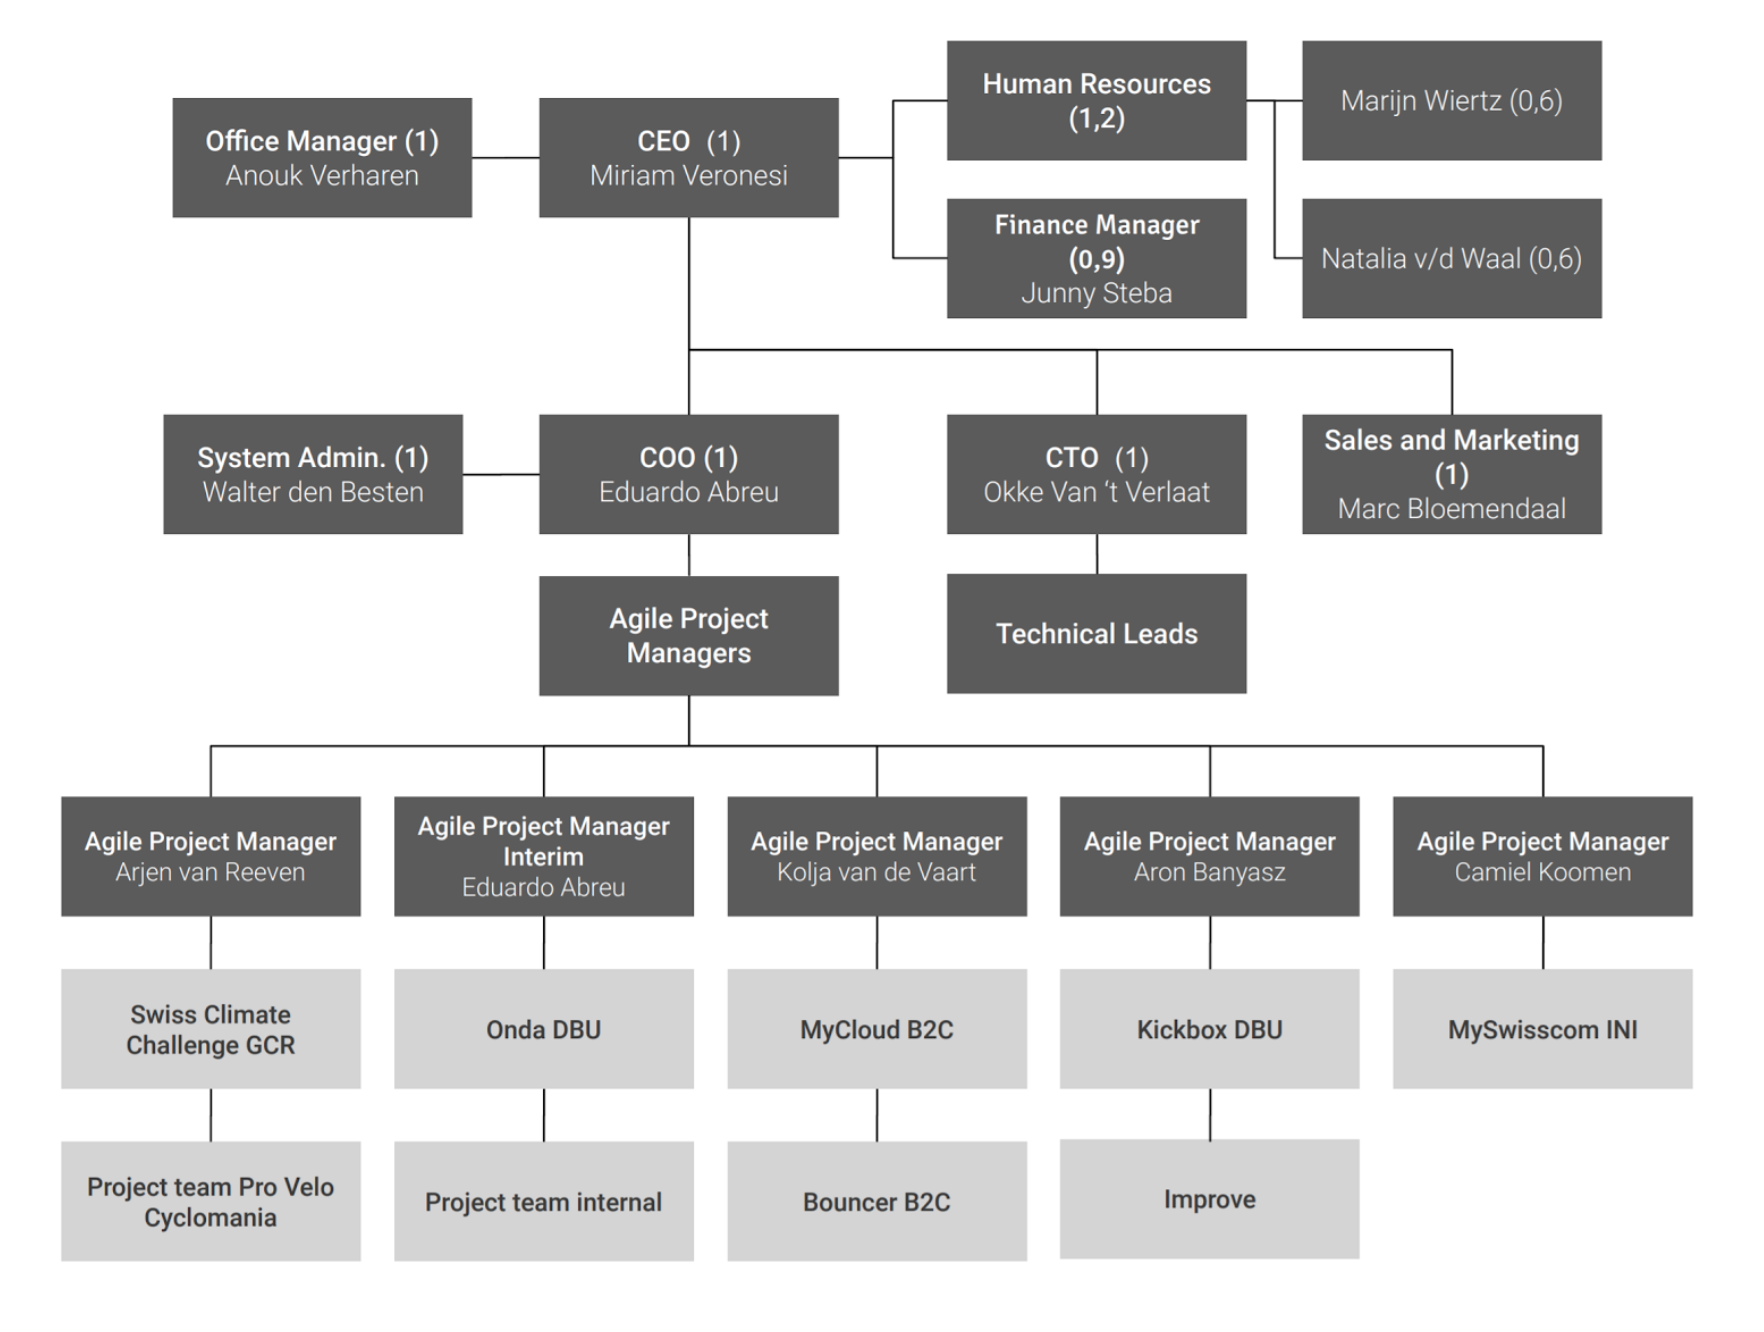
\includegraphics[width=14cm]{./chapter-1/organogram.png}
  \caption{Organogram van NGTI op 29-03-2021 \cite{ngti-organogram}.}
  \label{fig:ngti-organogram}
\end{figure}

NGTI is een dochterbedrijf van Swisscom \cite{swisscom-other-division}. Sinds maart 2021 is het bekend gemaakt dat Swisscom van plan is om een afdeling, Swisscom DevOps Center, te fuseren met NGTI. Omdat de fusie onzekerheid met zich meebrengt voor de structuur en manier hoe NGTI werkt, zal de situatie vóór de fusie aangehouden worden gedurende het afstuderen.

\section{Projecten van NGTI}\label{sec:ch1-projecten-van-ngti}
NGTI heeft een vrij breed portfolio met apps voor verschillende doeleinden. Een van deze apps is de Climate Challenge App \cite{ngti-swisscom-climate-challenge}. Met deze app kunnen gebruikers hun C02-voetafdruk en impact in kaart brengen. Er wordt bijgehouden hoeveel kilometer de gebruiker reist en met welk vervoersmiddel. De app is onderdeel van twee bestaande nieuwsapps, Blick en Bluewin \cite{swisscom-climate-challenge-integration}. Het doel is om de gebruiker aan te sporen om groener te reizen. Een screenshot van de app is te zien in \autoref{fig:swiss-climate-challenge-app}.

Een andere oplossing is de My Swisscom App \cite{ngti-my-swisscom-app}. Dit is een native app voor Android en iOS waarbij Swisscom-klanten hun contract kunnen bestellen, wijzigen of beëindigen. In de app kunnen klanten ook de dataverbruik zien en instellingen voor abonnementen wijzigen. Een screenshot van de app is te zien in \autoref{fig:my-swisscom-app}.

\begin{figure}[hbt!]
  \centering
  \begin{minipage}{0.45\textwidth}
      \centering
      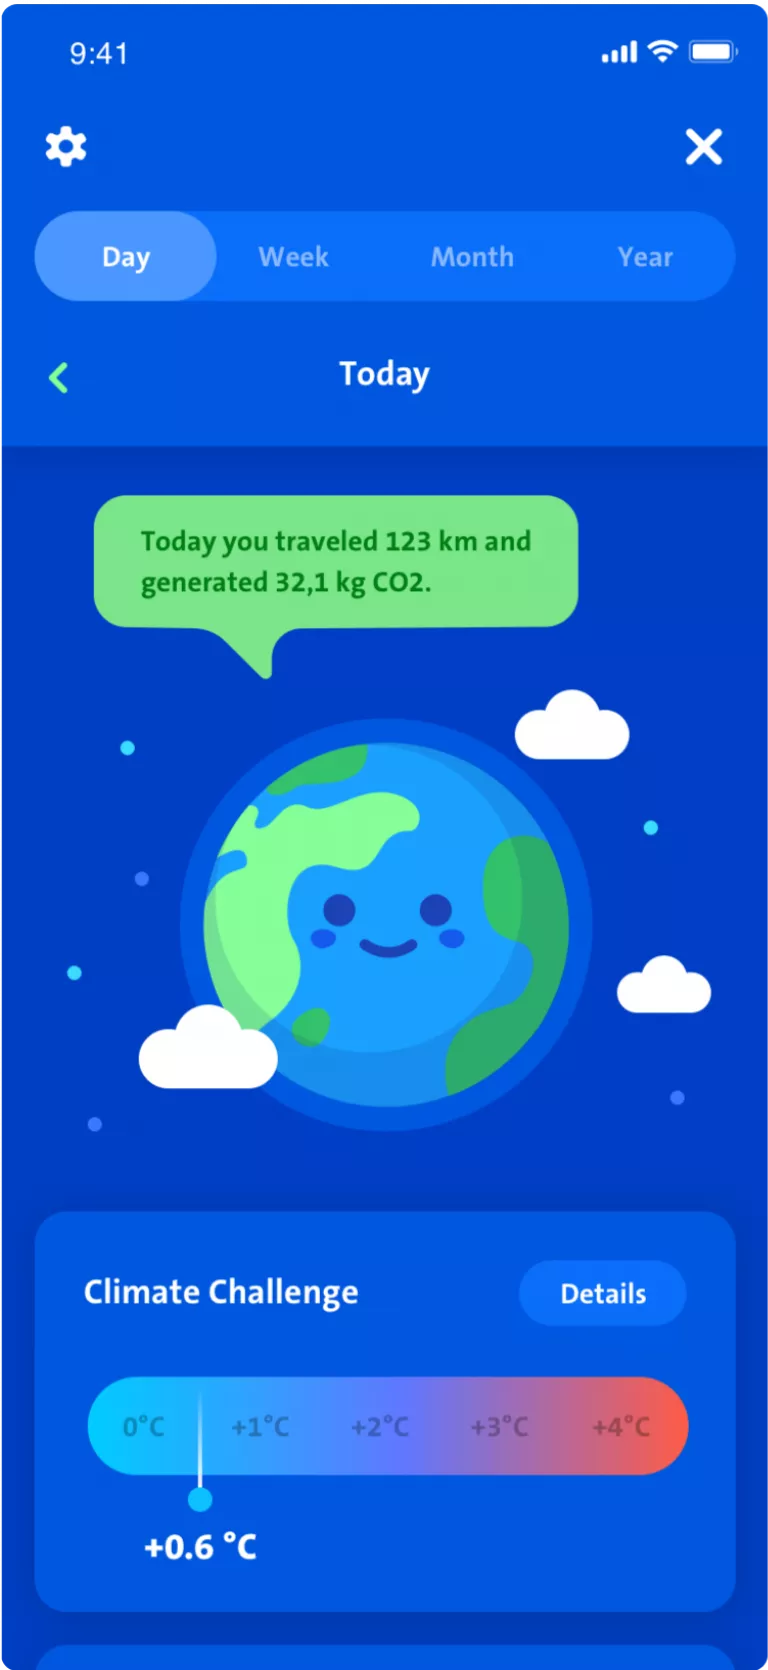
\includegraphics[width=0.65\textwidth]{./chapter-1/swiss-climate-challenge-app.png}
      \caption{Screenshot van de Swiss Climate Challenge app \cite{ngti-swisscom-climate-challenge}.}
      \label{fig:swiss-climate-challenge-app}
  \end{minipage}\hfill
  \begin{minipage}{0.45\textwidth}
      \centering
      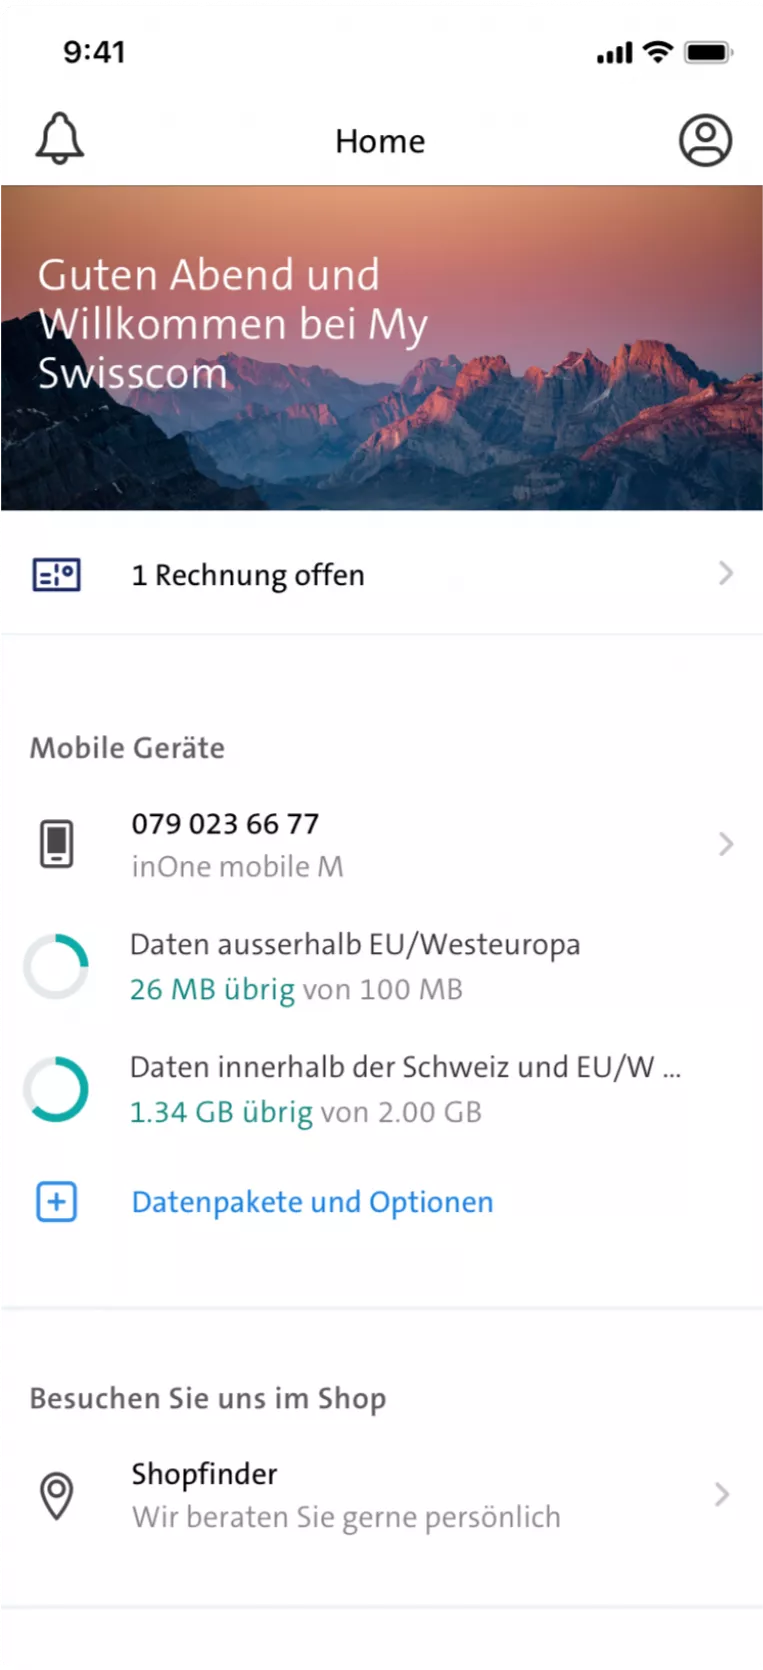
\includegraphics[width=0.65\textwidth]{./chapter-1/my-swisscom-app.png}
      \caption{Screenshot van de My Swisscom App \cite{ngti-my-swisscom-app}}
      \label{fig:my-swisscom-app}
  \end{minipage}
\end{figure}


\section{Tools die worden gebruikt}\label{sec:ch1-tools-die-gebruikt-worden}
Om productief te zijn, gebruikt NGTI een aantal tools en programma's om producten te maken en te communiceren met zowel collega's als klanten. De meest gebruikte en belangrijkste zijn Slack, Google Workspace, Zoom en Microsoft Teams.

\subsection{Slack}\label{subsec:slack}
Interne communicatie gaat via Slack. Het programma faciliteert collega's om elkaar met een lage instap te benaderen en berichten die voor het hele bedrijf relevant zijn te versturen. Ook zijn er 'channels' beschikbaar over specifieke onderwerpen, zoals: \textit{\#dev}, \textit{\#ios} en \textit{\#test-automation}.

\subsection{Google Workspace}\label{subsec:google-workspace}
Met Google Workspace kunnen bestanden en documenten gemaakt, opgeslagen en gedeeld worden. Dit is mogelijk via een browser waardoor werknemers geen software hoeven te installeren. NGTI gebruikt het ook om collaboratief en parallel te werken aan hetzelfde document.

\subsection{Microsoft Teams en Zoom}\label{subsec:microsoft-teams-en-zoom}
Voorheen werd Zoom alleen gebruikt om te videobellen met collega's en geïnterviewden. In de tijd van de pandemie is Zoom echter een belangrijke speler geworden om effectief samen te werken. Meetings zoals introducties van nieuwe collega's of demo's van producten worden online gehouden.

\section{Aanleiding opdracht}\label{sec:ch1-aanleiding-opdracht}
NGTI wilt de gebruikerservaring van haar apps verbeteren en een voorsprong hebben op haar concurrenten. Dit kan NGTI op een aantal manieren doen waarvan apps "slimmer"\space maken er een van is. Het slimmer maken houdt voor NGTI in dat de app bijvoorbeeld beter kan anticiperen wat de gebruiker wilt en nodig heeft op een gegeven moment. Dit kan onder andere door het toepassen van machine learning (ML). De opdracht kan verdeelt worden in twee onderdelen:

\begin{itemize}
  \item Onderzoek naar hoe een pipeline opgezet kan worden op een cloud computing platform door middel van een framework
  \item Onderzoek naar het maken van een platform-agnostische oplossing
\end{itemize}

Daarnaast zal een proof-of-concept (PoC) gemaakt worden om aan te tonen of het haalbaar is in de praktijk. Een diepere duik in het probleem en het definiëren van de onderdelen is te vinden in \autoref{chap:probleemanalyse}.